\documentclass[11pt]{standalone}
\usepackage[usenames]{color} %used for font color
\usepackage{amssymb} %maths
\usepackage{amsmath} %maths

\usepackage[no-math]{fontspec}
\setmainfont{Lato}
\usepackage{unicode-math}

\usepackage{tikz}
\usetikzlibrary{positioning}

% Farben definieren
\definecolor{background}{HTML}{F3F4F4}
\definecolor{inputneuron}{HTML}{CCDEE9}
\definecolor{outputneuron}{HTML}{005A94}

\begin{document}
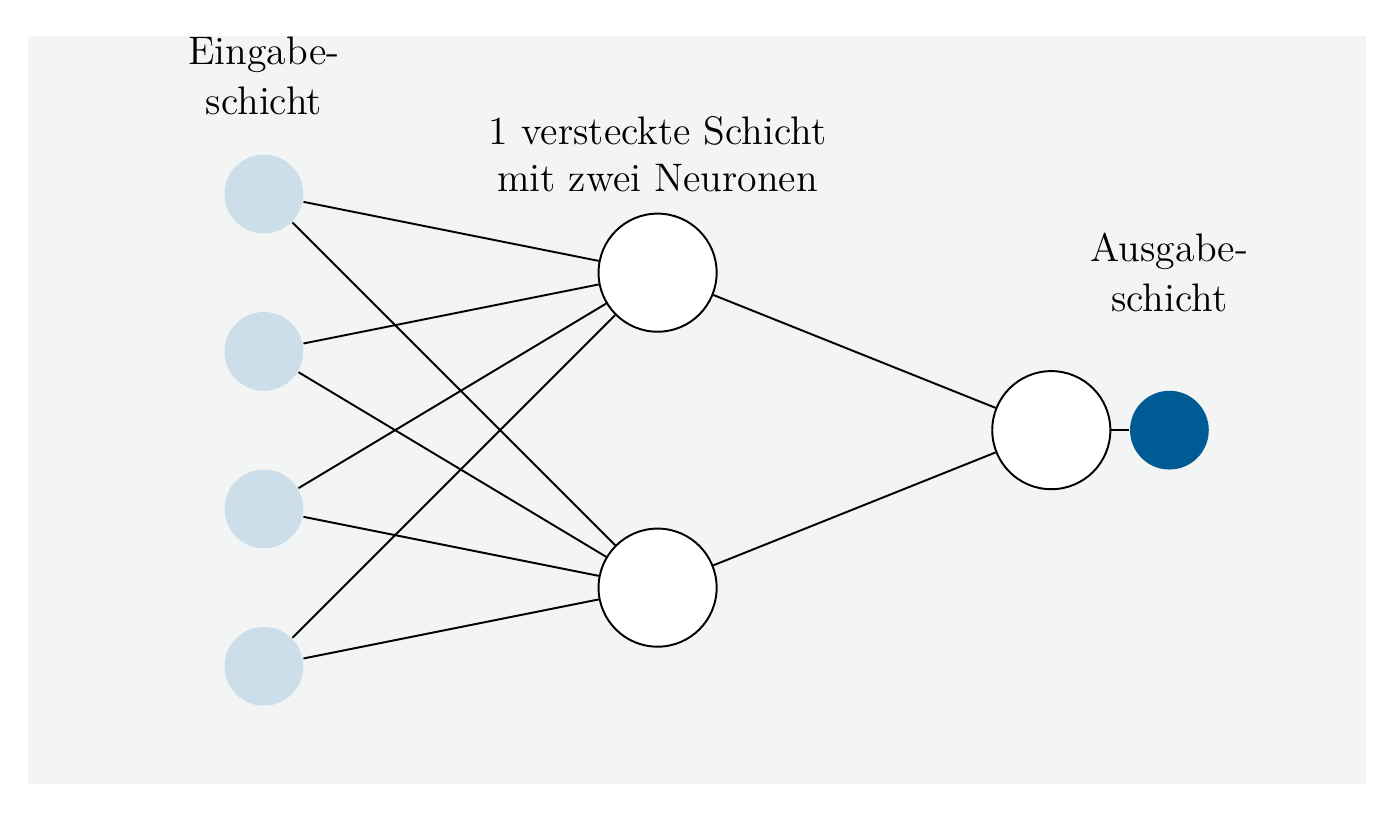
\begin{tikzpicture}[
    % Stile definieren
    neuron/.style={circle, minimum size=1cm, draw=black, line width=0.7pt},
    input neuron/.style={neuron, fill=inputneuron, draw=none},
    hidden neuron/.style={neuron, fill=white, minimum size=1.5cm},
    output neuron/.style={neuron, fill=outputneuron, draw=none},
    output circle/.style={circle, minimum size=1.5cm, draw=black, line width=0.7pt, fill=white},
    connection/.style={draw=black, line width=0.7pt}
]

% Hintergrund
\fill[background] (-3,-4.5) rectangle (14,5);

% Eingabeschicht (4 Neuronen)
\node[input neuron] (I1) at (0,3) {};
\node[input neuron] (I2) at (0,1) {};
\node[input neuron] (I3) at (0,-1) {};
\node[input neuron] (I4) at (0,-3) {};

% Verdeckte Schicht (2 Neuronen)
\node[hidden neuron] (H1) at (5,2) {};
\node[hidden neuron] (H2) at (5,-2) {};

% Ausgabeschicht (1 Neuron)
\node[output circle] (O1) at (10,0) {};
\node[output neuron] (O2) at (11.5,0) {};

% Verbindungen von Eingabeschicht zur verdeckten Schicht
\foreach \i in {1,...,4}
    \foreach \j in {1,2}
        \draw[connection] (I\i) -- (H\j);

% Verbindungen von versteckter Schicht zur Ausgabeschicht
\foreach \i in {1,2}
    \draw[connection] (H\i) -- (O1);

% Verbindung vom weißen Kreis zum blauen Kreis
\draw[connection] (O1) -- (O2);

% Beschriftungen
\node[font=\Large] at (5,3.8) {1 versteckte Schicht};
\node[font=\Large] at (5,3.2) {mit zwei Neuronen};

\node[font=\Large, align=center] at (0,4.5) {Eingabe-\\schicht};

\node[font=\Large, align=center] at (11.5,2) {Ausgabe-\\schicht};

\end{tikzpicture}
\end{document}
